\documentclass[a4paper,12pt]{article}

%%% Работа с русским языком
\usepackage{cmap}					% поиск в PDF
\usepackage{mathtext} 				% русские буквы в формулах
\usepackage[T2A]{fontenc}			% кодировка
\usepackage[utf8]{inputenc}			% кодировка исходного текста
\usepackage[english,russian]{babel}	% локализация и переносы

%%% Дополнительная работа с математикой
\usepackage{amsfonts,amssymb,amsthm,mathtools} % AMS
\usepackage{amsmath}
\usepackage{icomma} % "Умная" запятая: $0,2$ --- число, $0, 2$ --- перечисление

%% Номера формул
%\mathtoolsset{showonlyrefs=true} % Показывать номера только у тех формул, на которые есть \eqref{} в тексте.

%% Шрифты
\usepackage{euscript}	 % Шрифт Евклид
\usepackage{mathrsfs} % Красивый матшрифт

%% Свои команды
\DeclareMathOperator{\sgn}{\mathop{sgn}}

\usepackage{caption}
\usepackage{tabto}

%% Перенос знаков в формулах (по Львовскому)
\newcommand*{\hm}[1]{#1\nobreak\discretionary{}
{\hbox{$\mathsurround=0pt #1$}}{}}

%%% Работа с картинками
\usepackage{graphicx}  % Для вставки рисунков
\graphicspath{{images/}{images2/}}  % папки с картинками
\setlength\fboxsep{3pt} % Отступ рамки \fbox{} от рисунка
\setlength\fboxrule{1pt} % Толщина линий рамки \fbox{}
\usepackage{wrapfig} % Обтекание рисунков и таблиц текстом

%%% Работа с таблицами
\usepackage{array,tabularx,tabulary,booktabs} % Дополнительная работа с таблицами
\usepackage{longtable}  % Длинные таблицы
\usepackage{multirow} % Слияние строк в таблице


%%% Заголовок
\author{Документы и презентации в \LaTeX}
\title{2.1 Рисунки и таблицы}
\date{\today}

\begin{document} % конец преамбулы, начало документа
Пусть рис. \ref{fig:21} представляет положения Солнца $S$, Земли $T$ и Луны $L$, и пусть $\Theta$ есть центр тяжести Земли и Луны. Делаем следующие обозначения:

\begin{table}[h]
	\begin{center}
		\begin{tabular}{cccc}
    	Масса	& Солнца	& . . . . . &	$S$ \\ 
   		>>		& Земли		& . . . . . &	$T$ \\
   		>>		& Луны		& . . . . . &	$L$ \\
		\end{tabular}
	\end{center}
	\caption{Обозначения}
	\label{tab:designations}
\end{table}

Расстояние:
\[ S\Theta = \rho; ~ ST = \rho_1; ~ SL = \rho_2; ~ TL = r \]
тогда будет:
\begin{equation}
	\begin{aligned}
		T\Theta &= r_1 = \frac{L}{T + L} \cdot r \\
		L\Theta &= r_2 = \frac{T}{T + L} r
	\end{aligned}
	\label{eq:r1_r2}
\end{equation}

Составим теперь выражения ускорений, которые эти тела сообщают друг другу.

\begin{figure}[h]
	\begin{center}
		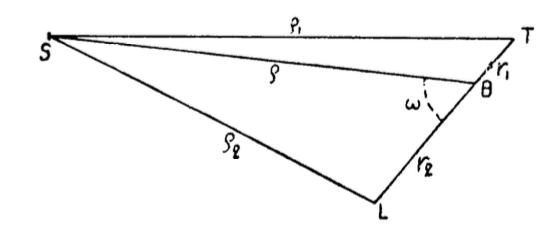
\includegraphics[scale = 1]{21.png}
		\caption{}
		\label{fig:21}
	\end{center}
\end{figure}

Солнце $S$ сообщает ускорения:
\[
	\begin{aligned}
		&\text{Земле:} & &f \cdot \frac{S}{\rho_1^2} & &\text{по направлению } &TS \\
		&\text{Луне:}  & &f \cdot \frac{S}{\rho_2^2} & &\text{ >> } \qquad \text{ >> } \qquad \quad \, &LS
	\end{aligned}
\]
вследствие чего точка $\Theta$ имеет ускорения:
\[
\begin{aligned}
	&\frac{T}{T + L} \cdot f \cdot \frac{S}{\rho_1^2} & &\text{по направлению, параллельному } &TS \\
	&\frac{L}{T + L} \cdot f \cdot \frac{S}{\rho_2^2} & &\text{ >> } \qquad \quad \text{ >> } \qquad \quad \quad \text{ >> }  &LS
\end{aligned}
\]

Ускорения Солнца, происходящие от притяжения Земли и Луны, соответственно, суть:
\[
\begin{aligned}
	&f \cdot \frac{T}{\rho_1^2} & &\text{по направлению } &ST \\
	&f \cdot \frac{L}{\rho_2^2} & &\text{ >> } \qquad \text{ >> } \qquad \quad \, &SL
\end{aligned}
\]
поэтому ускорение точки $\Theta$ относительно точки $S$ будет:
\[
\begin{aligned}
	\omega_1 &= f \cdot \frac{(S + T + L)}{T + L} \cdot \frac{T}{\rho_1^2} & &\text{по направлению параллельному } &TS \\
	\omega_2 &= f \cdot \frac{\text{ } S + T + L\text{ }}{T + L} \cdot \frac{L}{\rho_1^2} & &\text{ >> } \qquad \quad \text{ >> } \qquad \quad \quad \text{ >> }  &LS
\end{aligned}
\]


\begin{wrapfigure}{l}{0.5 \linewidth}
	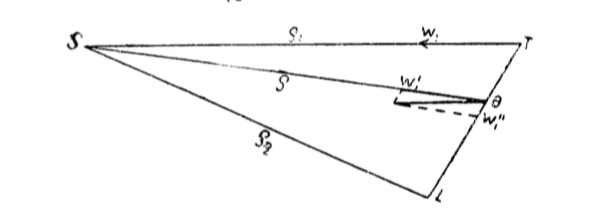
\includegraphics[width=\linewidth]{22.png}
	\caption{}
	\label{fig:22}
\end{wrapfigure}Разлагая эти ускорения, соответственно, по направлениям $\Theta S$ и $\Theta L$, получим, как легко видеть из подобия показанных на рис.\ref{fig:22} и \ref{fig:23} треугольников: 
\[
\begin{aligned}
	\omega'_1 &= \omega_1 \cdot \frac{\rho}{\rho_1} & &\text{по направлению } &\Theta S \\
	\omega''_1 &= \omega_1 \cdot \frac{r_1}{\rho_1} & &\text{ >> } \qquad \text{ >> } \qquad \quad \, &\Theta L\\
	\omega'_2 &= \omega_2 \cdot \frac{\rho}{\rho_2} & &\text{ >> } \qquad \text{ >> } \qquad \quad \, &\Theta S \\
	\omega''_2 &= \omega_2 \cdot \frac{r_2}{\rho_2} & &\text{ >> } \qquad \text{ >> } \qquad \quad \, &L \Theta 
\end{aligned}
\]\\
получим для ускорений точки $\Theta$ слагающие:
\[
\begin{aligned}
	W_1 = \omega'_1 + \omega'_2 = f \cdot \frac{S + T + L}{T + L} \cdot 
	\left[  T \cdot \frac{\rho}{\rho_1^3} + L \cdot \frac{\rho}{\rho_2^3}\right] &&\text{по } \Theta S \\
	W_2 = \omega''_1 + \omega''_2 = f \cdot \frac{S + T + L}{T + L} \cdot
	\left[  T \cdot \frac{r_1}{\rho_1^3} - L \cdot \frac{r_2}{\rho_2^3}\right] &&\text{по } \Theta L
\end{aligned}
\]

\begin{figure}[h]
	\begin{center}
		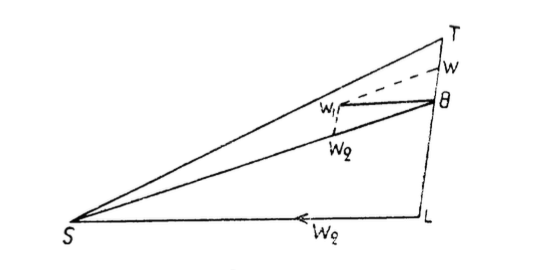
\includegraphics[scale = 1]{23.png}
		\caption{}
		\label{fig:23}
	\end{center}
\end{figure}

Заменив $r_1$ и $r_2$ их выражениями \eqref{eq:r1_r2} имеем:
\[
\begin{aligned}
	W_1 &= f \cdot \frac{S + T + L}{T + L} \cdot \rho \cdot
	\left[\frac{T}{\rho_1^3} + \frac{L}{\rho_2^3}\right]
	\text{по направлению } \Theta S \\
	W_2 &= f \cdot \frac{S + T + L}{(T + L)^2} \cdot T\cdot  L \cdot r
	\left[\frac{1}{\rho_1^3} - \frac{1}{\rho_2^3}\right]
	\text{по направлению } \Theta L
\end{aligned}
\]
Но
\[
\begin{aligned}
	\rho_1^2 &= \rho^2 + 2\rho \cdot \frac{L}{T + L} \cdot r \cos \omega + 
	\left(\frac{L}{T + L}\cdot r \right)^2 \\
	\rho_2^2 &= \rho^2 - 2\rho \; \; \; \frac{L}{T + L} \; \; \; r \cos \omega + 
	\left(\frac{T}{T + L} r \right)^2
\end{aligned}
\]
следовательно:
\[
\begin{aligned}
	\frac{1}{\rho_1^3} &= \frac{1}{\rho^3} \left[ 1 + 3\frac{L}{T + L} \cos \omega + \left( \frac{L}{T + L} r \right)^2\left( -\frac{3}{2} + \frac{15}{2} \cos^2 \omega \right) + \dots \right] \\
	\frac{1}{\rho_2^3} &= \frac{1}{\rho^3} \left[ 1 + 3\frac{T}{T + L} \cos \omega + \left( \frac{T}{T + L} r \right)^2\left( -\frac{3}{2} + \frac{15}{2} \cos^2 \omega \right) + \dots \right] 
\end{aligned}
\]
Подставляя эти выражения, имеем:
\[
\begin{aligned}
	W_1 &= f \cdot \frac{S + T + L}{\rho^2}
	\left[ 1 + \frac{T \cdot L}{(T + L)^2} \cdot \frac{r^2}{\rho^2} 
	\left( -\frac{3}{2} + \frac{15}{2} \cos^2 \omega \right) + \dots \right] \\
	W_2 &= f \cdot \frac{S + T + L}{\rho^2}
	\left[ -3 \cdot \frac{T \cdot L}{(T + L)^2} \cdot \frac{r^2}{\rho^2} 
	\cos \omega + \dots \right]
\end{aligned}
\]
Но отношения
\[
	\frac{L}{T + L} \approx \frac{1}{80}; \quad 
	\frac{r}{\rho} \approx \frac{1}{400}; \quad 
	\left( \frac{r}{\rho} \right)^2 = \frac{1}{160000}
\]
поэтому будет 
\[
	\frac{T \cdot L}{(T + L)^2} \cdot \frac{r^2}{\rho^2} \approx \frac{1}{12800000}
\]
и члены, содержащие этот множитель, могут быть отброшены, так что будет:
\[
\begin{aligned}
	W_1 &= f \cdot \frac{S + T + L}{\rho^2} ~ \text{ по направлению } \Theta S \\
	W_2 &= 0 ~ \text{ по направлению } \Theta L
\end{aligned}
\]

Отсюда следует, что точка $\Theta$ движется вокруг Солнца по эллиптической орбите по законам Кеплера.

Рассмотрим теперь ускорение Луны по отношению к Земле, для чего к ускорениям, сообщаемым Луне Солнцем и Землею, надо присовокупить ускорение, равное и противоположное ускорению Земли, происходящему от действия Солнца и Луны. Поступив подобно предыдущему, получим:
\[
\begin{aligned}
	f \cdot \frac{T + L}{r^2} & + f \cdot S \left[ \frac{r_2}{\rho_2^3}  + \frac{r_1}{\rho_1^3} \right] \text{ по направлению } L \Theta  \\	
	f \cdot & S \cdot \rho \left[ \frac{1}{\rho_2^3} - \frac{1}{\rho_1^3} \right] \text{ параллельно } \Theta S
\end{aligned}
\]
положим:
\[
	T + L = \mu; ~ S = M
\]

\newpage

\listoftables

\listoffigures

\end{document} % конец документа